%
%!TEX root = ../../../hp3D_user_guide.tex
%

%--------------------------------------------------------------------

\subsection{DPG ultraweak implementation}
\label{sec:poisson-ultraweak}

The ultraweak formulation is based on the first-order system:
\begin{align*}
	\bs \sigma - \grad u &= \bs 0 , \\
	- \div \bs \sigma &= f .
\end{align*}

The broken ultraweak formulation is then given by:
\[
\left\{
\begin{array}{llll}
	\hat u \in H^{1/2}(\Gamma_h): \hat u = u_0 \text{ on } \Gamma,\,
	\hat{\sigma}_n \in H^{-1/2}(\Gamma_h),\,
	u \in L^2(\Omega),\,
	\bs \sigma \in \bs{L^2}(\Omega) , \\[5pt]
	(\bs \sigma, \bs \tau) + (u, \nablah \cdot \bs \tau)
	- \lb \hat u, \bs \tau \cdot \bs n \rb_{\Gamma_h}
	+ (\bs \sigma, \nablah v)
	- \lb \hat{\sigma}_n , v \rb_{\Gamma_h}
	= (f,v) \, , \
	v \in H^1(\Omega_h), 
	\bs \tau \in H(\tdiv; \Omega_h) \, .
\end{array}
\right.
\]

The DPG ultraweak implementation differs from the primal DPG implementation mostly in the \routine{elem} routine. As before, the static condensation of the Riesz representation of the residual is done at the element level (cf.~Section~\ref{sec:poisson-primal}). This model problem employs the adjoint graph norm as a test norm for the ultraweak DPG implementation:
\[
	\| (v,\bs \tau) \|^2_\test := 
	\| \nablah v + \bs \tau \|^2 + \| \nablah \cdot \bs \tau \|^2
	+ \| v \|^2 + \| \bs \tau \|^2 .
\]

The implementation is provided in \file{problems/POISSON/ULTRAWEAK\_DPG}.

\begin{lstlisting}[caption=\file{POISSON/ULTRAWEAK\_DPG/input/physics} input file.]
100000               MAXNODS, nodes anticipated
4                    NR_PHYSA, physics attributes
trace_a contin  1    H1 variable
trace_b normal  1    H(div) variable
field    discon  1   L2 variable
grad     discon  3   L2 Variable
\end{lstlisting}

In the ultraweak formulation, there are four physics unknowns: $\hat u$, $\hat{\sigma}_n$, $u$, $\bs \sigma$; i.e.~\code{\var{NR\_PHYSA}=4}. The variables are defined in the \file{physics} file and the continuous trace $\hat u$ and the normal trace $\hat \sigma_n$ are specified as such by setting \code{\var{PHYSAi(1:2)}=.true.}. As before, the DPG \routine{elem} routine can be split into three distinct steps:

\begin{minipage}{0.48\textwidth}
\begin{enumerate}
	\itemsep -10pt
	\item Element integration \vspace{-15pt}
	\begin{itemize}
		\itemsep -8pt
		\item Stiffness: $\mr B$
		\item Load: $\mr l$
		\item Gram matrix: $\mr G$
	\end{itemize}
	\item Boundary integration \vspace{-15pt}
	\begin{itemize}
		\itemsep -8pt
		\item Stiffness: $\mr{\hat B_{1,1}, \hat B_{1,2}, \hat B_{2,1}, \hat B_{2,2}}$
	\end{itemize}
	\item Constructing DPG linear system \vspace{-15pt}
	\begin{itemize}
		\itemsep -8pt
		\item Dense linear algebra
		\item {Statically condensed system\\[-5pt] 
		stored in \var{ALOC}, \var{BLOC}}
	\end{itemize}
\end{enumerate}
\end{minipage}%
\begin{minipage}{0.48\textwidth}
\begin{figure}[H]
	\centering
		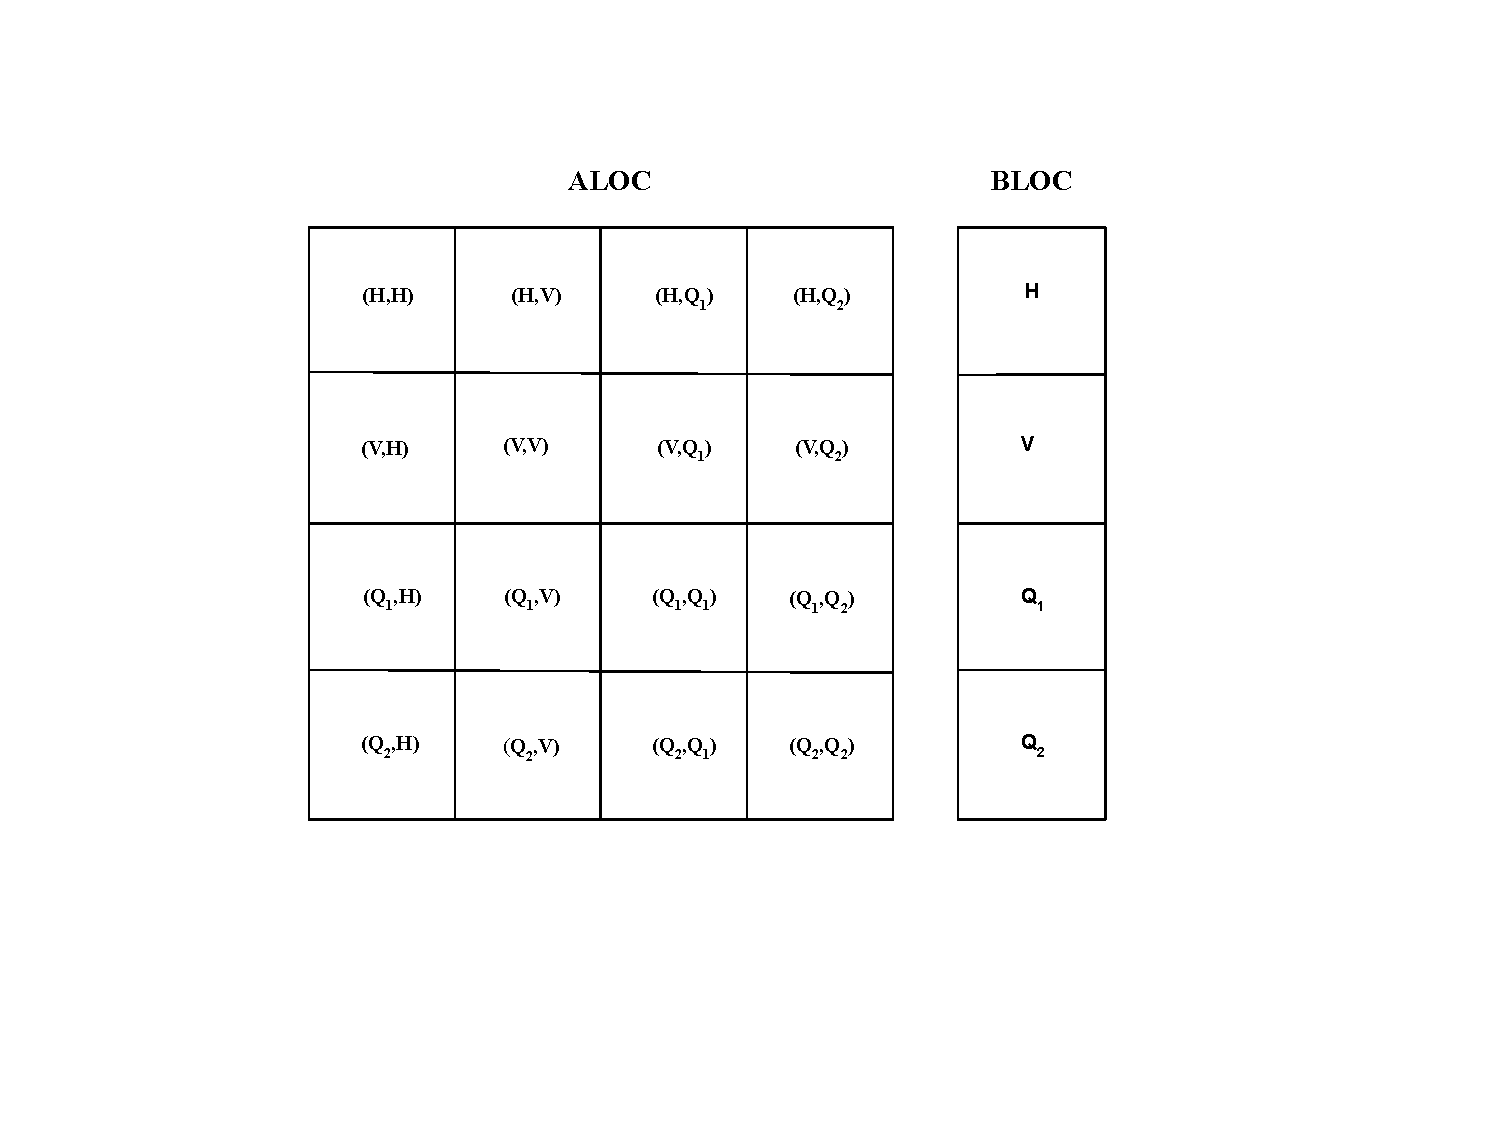
\includegraphics[scale=0.5]{ALOC_UW.pdf}
	\caption*{Element-local system.}
\end{figure}
\end{minipage}

\vskip 5pt
%\begin{minipage}[t]{0.60\textwidth}
%%Recall the statically condensed system\\[-5pt]
%(cf.~Appendix~\ref{chap:dpg}): \vspace{-10pt}
%\[
%  \var{stiff\_ALL}^* G^{-1} \var{stiff\_ALL} = \var{stiff\_ALL}^* G^{-1} \var{bload\_H} 
%\]
%\end{minipage}
\begin{minipage}[t]{\textwidth}
Auxiliary local variables: \vspace{-10pt}
\begin{itemize}
	\itemsep -8pt
	\item \var{stiff\_HH} $\leftarrow \mr{\hat B_{1,1}}$
	\item \var{stiff\_HV} $\leftarrow \mr{\hat B_{1,2}}$
	\item \var{stiff\_HQ1} $\leftarrow \mr{B_{1,3}}$
	\item \var{stiff\_HQ2} $\leftarrow \mr{B_{1,4}}$
	\item \var{stiff\_VH} $\leftarrow \mr {\hat B_{2,1}}$
	\item \var{stiff\_VV} $\leftarrow \mr{\hat B_{2,2}}$
	\item \var{stiff\_VQ1} $\leftarrow \mr{B_{2,3}}$
	\item \var{stiff\_VQ2} $\leftarrow \mr{B_{2,4}}$
	
	\item \var{bload\_H} $\leftarrow \mr {\left[ {l} \, | \, 0\right]}^T$
	\item \vskip 4pt \var{stiff\_ALL} $\leftarrow \left[\begin{array}{c|c|c|c|c}
	\hat B_{1,1} \, | \, & \hat B_{1,2} \, | \, & B_{1,3} \, | \, & B_{1,4} \, | \, & \text{l} \\ \hline
	\hat B_{2,1} \, | \, & \hat B_{2,2} \, | \, & B_{2,3} \, | \, & B_{2,4} \, | \, & 0
	\end{array} \right]$
\end{itemize}
\end{minipage}

The preliminary setup for the ultraweak formulation is similar to the setup of the primal DPG implementation with additional memory allocation for additional unknowns and test functions. The element integration routine for the ultraweak DPG formulation is given by the following code:
\begin{lstlisting}[mathescape,caption=\file{POISSON/ULTRAWEAK\_DPG/}\routine{elem}: element integration]
!..use the enriched order to set the quadrature
   INTEGRATION = NORD_ADD ! $\triangle p \in \{1,2,...\}$
   call set_3D_int_DPG(etype,norder,norient_face, nrint,xiloc,waloc)

!..loop over integration points
   do l=1,nrint

!..coordinates and weight of this integration point
      xi(1:3) = xiloc(1:3,l)
      wa = waloc(l)

!..H1 shape functions (for geometry)
      call shape3DH(etype,xi,norder,norient_edge,norient_face, nrdof,shapH,gradH)

!..L2 shape functions
      call shape3DQ(etype,xi,norder, nrdof,shapQ)

!..discontinuous H1 shape functions
      call shape3HH(etype,xi,nordP, nrdof,shapHH,gradHH)
!..discontinuous H(div) shape functions
      call shape3VV(etype,xi,nordP, nrdof,shapVV,divVV)

!..geometry map
      call geom3D(Mdle,xi,xnod,shapH,gradH,NrdofH, x,dxdxi,dxidx,rjac,iflag)

!..integration weight
      weight = rjac*wa

!..get the RHS
      call getf(Mdle,x, fval)

!..1st loop through enriched H1 test functions
      do k1=1,NrdofHH
!..Piola transformation
         v = shapHH(k1)
         dv(1:3) = gradHH(1,k1)*dxidx(1,1:3) &
                  + gradHH(2,k1)*dxidx(2,1:3) &
                  + gradHH(3,k1)*dxidx(3,1:3)

!..accumulate load vector: $\mr{(f,v)}$
         bload_H(k1) = bload_H(k1) + fval*v*weight

!..loop through L2 trial functions
         do k2=1,NrdofQ
!..loop over components of $\sigma$
            do ivar = 1,3
               n1 = k1; n2 = (k2 - 1)*3 + ivar
               sig = ZERO
!..Piola Transform for $\mr{{ivar}^{th}}$ L2 component of $\sigma$
               sig(ivar) = shapQ(k2) / rjac
!..accumulate stiffness: $\mr{(\bs \sigma,\nabla v)}$
               stiff_HQ2(n1,n2) = stiff_HQ2(n1,n2) + weight * &
               	                 (sig(1)*dv(1) + sig(2)*dv(2) + sig(3)*dv(3))
            enddo; enddo !..end of loop through L2 trial functions

!..2nd loop through enriched H1 test functions for Gram matrix
         do k2=k1,NrdofHH
!..Piola transformation
            q = shapHH(k2)
            dq(1:3) = gradHH(1,k2)*dxidx(1,1:3) &
                     + gradHH(2,k2)*dxidx(2,1:3) &
                     + gradHH(3,k2)*dxidx(3,1:3)

!..determine index in triangular packed format            
            k = nk(k1,k2)
!..accumulate components of Gram matrix corresponding to $\mr{v}$
            aux = q*v + (dq(1)*dv(1) + dq(2)*dv(2) + dq(3)*dv(3))
            gramP(k) = gramP(k) + aux*weight
         enddo !..end of 2nd loop through enriched H1 test functions

!..cross terms for  graph norm
         do k2 = 1,NrdofVV
            tau_a(1:3) = ( dxdxi(1:3,1) * shapVV(1,k2)       &
                           + dxdxi(1:3,2) * shapVV(2,k2)     &
                           + dxdxi(1:3,3) * shapVV(3,k2) ) / rjac

            k = nk(k1,NrdofHH+k2)
!..accumulate components of Gram matrix corresponding to inner products involving $\mr{v}$ and $\mr{\bs \tau}$
            aux = dv(1) * tau_a(1) + dv(2) * tau_a(2) + dv(3) * tau_a(3)
            gramP(k) = gramP(k) + aux * weight
         enddo
      enddo !..end of 1st loop through enriched H1 test functions

!..loop over discontinuous H(div) test functions
      do k1=1,NrdofVV
!..Piola transformation
         divtau_a = divVV(k1)/rjac
         tau_a(1:3) = ( dxdxi(1:3,1) * shapVV(1,k1)      &
                       + dxdxi(1:3,2) * shapVV(2,k1)     &
                       + dxdxi(1:3,3) * shapVV(3,k1) ) / rjac
         
         do k2=1,NrdofQ
            u = shapQ(k2) / rjac !..Piola transformation

!..accumulate stiffness: $\mr{(u,\nabla \cdot \bs \tau)}$
            stiff_VQ1(k1,k2) = stiff_VQ1(k1,k2) + weight*(u * divtau_a)

            do ivar = 1,3
               sig = ZERO
               sig(ivar) = shapQ(k2)/rjac  ! Piola transform for the $\mr{{ivar}^{th}}$ component
               n1 = k1; n2 = (k2 - 1)*3 + ivar
!..accumulate stiffness: $\mr{(\bs \sigma,\bs \tau)}$
               stiff_VQ2(n1,n2) = stiff_VQ2(n1,n2) + weight * & 
                                  (tau_a(1)*sig(1) + tau_a(2)*sig(2) + tau_a(3)*sig(3))
            enddo; enddo ! end of loop over L2 trial functions

!..Gram matrix contribution for H(div) inner product
         do k2=k1,NrdofVV
!..Piola transformation
            divtau_b = divVV(k2)/rjac
            tau_b(1:3) = ( dxdxi(1:3,1) * shapVV(1,k2)       &
                           + dxdxi(1:3,2) * shapVV(2,k2)     &
                           + dxdxi(1:3,3) * shapVV(3,k2) ) / rjac
!
            k = nk(k1 + NrdofHH,k2 + NrdofHH)
            aux = divtau_a * divtau_b + 2.d0 * 
                  (tau_a(1)*tau_b(1) + tau_a(2)*tau_b(2) + tau_a(3)*tau_b(3))
            gramP(k) = gramP(k) +  weight * aux
         enddo; enddo !..end of loop over H(div) test functions
   enddo !..end of loop over integration points
\end{lstlisting}

Next, we provide the code performing the boundary integration:
\begin{lstlisting}[mathescape,caption=\file{POISSON/ULTRAWEAK\_DPG/}\routine{elem}: boundary integration]
!..loop through element faces
   do ifc=1,nrf

!..sign factor to determine the outward normal unit vector
      nsign = nsign_param(etype,ifc)

!..face type
      ftype = face_type(etype,ifc)

!..face order of approximation
      call face_order(etype,ifc,norder, norderf)

!..set 2D quadrature
      INTEGRATION = NORD_ADD
      call set_2D_int_DPG(ftype,norderf,norient_face(ifc), nrint,tloc,wtloc)

!..loop through integration points
      do l=1,nrint

!..face coordinates
         t(1:2) = tloc(1:2,l)

!..face parametrization
         call face_param(etype,ifc,t, xi,dxidt)

!..determine discontinuous H1 shape functions
         call shape3HH(etype,xi,nordP, nrdof,shapHH,gradHH)
!..discontinuous H(div) shape functions
         call shape3VV(etype,xi,nordP, nrdof,shapVV,divVV)

!..determine element H1 shape functions (for geometry)
         call shape3DH(etype,xi,norder,norient_edge,norient_face, nrdof,shapH,gradH)

!..determine H(div) shape functions (for fluxes) on face
         call shape3DV(etype,xi,norderi,norient_face, nrdof,shapV,divV)

!..geometry map
         call bgeom3D(Mdle,xi,xnod,shapH,gradH,NrdofH,dxidt,nsign, &
                       x,dxdxi,dxidx,rjac,dxdt,rn,bjac)
!..integration weight
         weight = bjac*wtloc(l)

!..loop through enriched H1 test functions
         do k1=1,NrdofHH
            v = shapHH(k1)

!..loop through H(div) trial functions on face
            do k2=1,NrdofVi_b
!..Piola transformation
               s(1:3) = ( dxdxi(1:3,1)*shapV(1,k2) &
                         + dxdxi(1:3,2)*shapV(2,k2) &
                         + dxdxi(1:3,3)*shapV(3,k2) ) / rjac
!..normal component
               sn = s(1)*rn(1) + s(2)*rn(2) + s(3)*rn(3)

!..accumulate stiffness: $\mr{- \left\langle \hat{\sigma}_n,v \right\rangle}$
               stiff_HV(k1,k2) = stiff_HV(k1,k2) - sn*v*weight
            enddo !..end of loop through H(div) trial functions on face
         enddo !..end of loop through enriched H1 test functions

!..loop through enriched H(div) test functions
         do k1=1,NrdofVV
!..Piola Transform
            tau_a(1:3) = ( dxdxi(1:3,1) * shapVV(1,k1)      &
                          + dxdxi(1:3,2) * shapVV(2,k1)     &
                          + dxdxi(1:3,3) * shapVV(3,k1) ) / rjac
            tn = tau_a(1)*rn(1) + tau_a(2)*rn(2) + tau_a(3)*rn(3)

            do k2=1,NrdofVi_a
!..accumulate stiffness: $\mr{-\left\langle \hat u, \tau \cdot n \right\rangle}$
               u_hat = shapH(k2)
               stiff_VH(k1,k2) = stiff_VH(k1,k2) - weight * tn * u_hat
            enddo !..end of loop through H1 trial functions
         enddo !..end of loop through enriched H(div) test functions
      enddo !..end of loop through integration points
   enddo !..end of loop through element faces
\end{lstlisting}

Finally, the code performing the construction of the DPG linear system:
\begin{lstlisting}[mathescape,caption=\file{POISSON/ULTRAWEAK\_DPG/}\routine{elem}: constructing DPG linear system.]
   allocate(stiff_ALL(NrTest,NrTrial+1))
   stiff_ALL = ZERO

!  Total test/trial DOFs of the element
   i1 = NrdofHH; i2 = NrdofVV; j1 = NrdofVi_a; j2 = NrdofVi_b; j3 = NrdofU; j4 = NrdofS

!..Copy stiffness and load into one matrix
   stiff_ALL(1:i1,1:j1) = stiff_HH
   stiff_ALL(1:i1,j1+1:j1+j2) = stiff_HV
   stiff_ALL(1:i1,j1+j2+1:j1+j2+j3) = stiff_HQ1
   stiff_ALL(1:i1,j1+j2+j3+1:j1+j2+j3+j4) = stiff_HQ2

   stiff_ALL(i1+1:i1+i2,1:j1) = stiff_VH
   stiff_ALL(i1+1:i1+i2,j1+1:j1+j2) = stiff_VV
   stiff_ALL(i1+1:i1+i2,j1+j2+1:j1+j2+j3) = stiff_VQ1
   stiff_ALL(i1+1:i1+i2,j1+j2+j3+1:j1+j2+j3+j4) = stiff_VQ2

   stiff_ALL(1:i1+i2,j1+j2+j3+j4+1) = bload_H

!..A. Compute Cholesky factorization of Gram Matrix, $\mr{G=U^T U (=LL^T)}$
   call DPPTRF('U',NrTest,gramP,info)

!..B. Solve triangular system to obtain $\mr{\tilde{B}}$, $\mr{(LX=) U^T X = [B|l]}$
   call DTPTRS('U','T','N',NrTest,NrTrial+1,gramP,stiff_ALL,NrTest,info)

   allocate(raloc(NrTrial+1,NrTrial+1)); raloc = ZERO

!..C. Matrix multiply: $\mr{B^T G^{-1} B (=\tilde{B}^T \tilde{B})}$
   call DSYRK('U','T',NrTrial+1,NrTest,ZONE,stiff_ALL,NrTest,ZERO,raloc,NrTrial+1)

!..D. Fill lower triangular part of Hermitian matrix using the upper triangular matrix $\mr{\tilde B^T \tilde B}$
   do i=1,NrTrial
      raloc(i+1:NrTrial+1,i) = raloc(i,i+1:NrTrial+1)
   enddo
   
!..raloc has now all blocks of the stiffness and load:
!  $r_{\text{aloc}} =   \var{ALOC(1,1)} \quad \var{ALOC(1,2)} \quad \var{ALOC(1,3)} \quad \var{ALOC(1,4)} \quad\var{BLOC(1)}$
!         $\, \var{ALOC(2,1)} \quad \var{ALOC(2,2)} \quad \var{ALOC(2,3)} \quad \var{ALOC(2,4)} \quad \var{BLOC(2)}$
!         $\, \var{ALOC(3,1)} \quad \var{ALOC(3,2)} \quad \var{ALOC(3,3)} \quad \var{ALOC(3,4)} \quad \var{BLOC(3)}$
!         $\, \var{ALOC(4,1)} \quad \var{ALOC(4,2)} \quad \var{ALOC(4,3)} \quad \var{ALOC(4,4)} \quad \var{BLOC(4)}$
\end{lstlisting}
